\section{Расчёт свойств потока}

В отличии от функций расчета PVT (физико-химических свойств флюидов) функции расчета свойства потока учитывают дополнительные параметры потока флюидов - $Q$ - дебит, объемный расход флюидов, $f_w$ - обводненность, $R_p$ - газовый фактор. В функциях свойств потока используется префикc \mintinline{vb.net}{MF_}.

Параметры потока, такие как расход ГЖС, доля газа в потоке, вязкость ГЖС важны для расчета и анализа работы скважин и скважинного оборудования.


\subsection{MF\_qmix\_m3day – расход газожидкостной смеси}

Функция позволяет рассчитать объемный расход газожидкостной смеси при заданных термобарических условиях. Объемный расход ГЖС важен например для подбора УЭЦН в скважине, так как именно определяет в какой точке характеристики УЭЦН будет работать. При наличии свободного газа в потоке расход ГЖС может быть значительно больше расхода жидкости на поверхности фиксируемого расходомером.
$$Q_{mix,rc} = Q_{w,sc} B_w(P,T) + Q_{o,sc} B_o(P,T)  + Q_{o,sc}  (R_p - R_s(P,T)) B_g(P,T) $$

Расход ГЖС определяется как сумма расходов отдельных фаз, приведенных к соответствующим термобарическим условиям, с учетом того, что часть газа будет растворена в нефти.

\putlisting{listings/MF_q_mix_rc_m3day.lst}

\subsection{MF\_rhomix\_kgm3 – плотность газожидкостной смеси}

Функция позволяет рассчитать плотность газожидкостной смеси при заданных термобарических условиях. 
$$\rho_{mix,rc} = \left( \frac{\rho_{w,sc}}{B_w} f_w + \frac{\rho_{o,sc} +r_s \rho_{g,sc} }{B_o}(1-f_w) \right) (1-f_g) + \frac{ \rho_{g,sc} }{B_g} f_g $$

\putlisting{listings/MF_Rhomix_kgm3.lst}

\subsection{MF\_gas\_fraction\_d – доля газа в потоке}

Функция расчёта доли свободного газа в потоке (без учёта проскальзывания) в зависимости от термобарических условий для заданного флюида. 
$$f_g = \frac{Q_{g,rc}}{Q_{mix,rc}} $$
Доля газа в потоке является одним из ключевых параметров ограничивающих производительность систем механизированной добычи - ЭЦН и других насосов.

\putlisting{listings/MF_gas_fraction_d.lst}

\subsection{MF\_p\_gas\_fraction\_atma – целевое давления для заданной доли газа в потоке}
Функция расчёта давления при котором достигается заданная доля свободного газа в потоке (без учёта проскальзывания). 
Значение давления при котором достигается определённая доля газа в потоке может быть найдено из решения уравнения, определяющего долю газа. 
$$f_g = \frac{Q_{g,rc}(P,T)}{Q_{mix,rc}(P,T)} $$
Решение в \unf реализовано итеративное, методом деления отрезка пополам (дихотомия). При вызове функции пересчитывается состояние смеси с различными термобарическими условиями. Поэтому расчёт проводится относительно медленно. 

\putlisting{listings/MF_p_gas_fraction_atma.lst}

\subsection{MF\_rp\_gas\_fraction\_m3m3 – целевой газовый фактор для заданной доли газа в потоке}
Функция расчёта газового фактора $R_p$ при котором достигается заданная доля свободного газа в потоке (без учёта проскальзывания) . 
Значение давления при котором достигается определённая доля газа в потоке может быть найдено из решения уравнения, определяющего долю газа. 
$$f_g = \frac{Q_{g,rc}(P,T,R_p)}{Q_{mix,rc}(P,T,R_p)} $$
Решение в \unf реализовано итеративное, методом деления отрезка пополам (дихотомия). При вызове функции пересчитывается состояние смеси с различными термобарическими условиями. Поэтому расчёт проводится относительно медленно. 

\putlisting{listings/MF_rp_gas_fraction_m3m3.lst}

\section{Сепарация газа в скважине}
В скважинах оборудованных системами механизированной добычи нефти важную роль играет процесс сепарации газа на приёме насоса. Под сепарацией газа понимается отделение части свободного газа из потока и перенаправление его по отдельному гидравлическому каналу на поверхность. В результате сепарации газа меняются свойства флюида, поступающего в насос и НКТ выше насоса. В частности меняются давление насыщения и газосодержание при давлении насыщения для флюида после сепарации. Более детальные модели флюида и сепарации могут показать, что при сепарации может поменяться и другие параметры - например состав газа после разгазирования. В модели нелетучей нефти реализованной в \unf{} эти эффекты не учитываются.

Оценка величины сепарации может быть проведена приведёнными ниже функциями.

\subsection{MF\_ksep\_natural\_d – естественная сепарация газа}
Функция рассчитывает естественную сепарацию газа на приёме насоса в скважине с использованием корреляции Маркеса \cite{Marquez_2003} . Результат - безразмерная величина в диапазоне от 0 до 1. 

\putlisting{listings/MF_ksep_natural_d.lst}

\subsection{MF\_ksep\_gasseparator\_d – сепарация газа роторным газосепаратором}
Функция рассчитывает сепарацию газа с использованием роторного газосепаратора, являющегося обычно частью компоновки УЭЦН. Данный расчет основан на результатах испытания характеристик роторных газосепараторов, выполненных в РГУ нефти и газа имени И.М.Губкина \cite{SPE_117415_2008}. 

Следует отметить, что несмотря на хорошее соответствие промысловых исследований и расчетов с использованием корреляции для естественной и искусственной сепарации \cite{SPE_117415_2008} к результатам стендовых исследований стоит относится с осторожностью. Основой осторожности могут быть следующие соображения: характеристики различных газосепараторов достаточно сильно отличаются друг от друга - есть удачные конструкции и не очень, при этом результаты стендовых испытаний доступны только для ограниченного набора конструкций, стендовые условия достаточно сильно отличаются от скважинных - ниже давление, другие модельные рабочие жидкости, точно оценить коэффициент сепарации газосепаратора в промысловых условиях затруднительно - набор таких данных для сравнения ограничен. 

Тем не менее изучение результатов стендовых испытаний полезно при проведении расчетов и развивает инженерную интуицию. 

\putlisting{listings/MF_ksep_gasseparator_d.lst}


\subsection{MF\_ksep\_total\_d – общая сепарация газа}

Функция рассчитывает полную сепарацию газа на приёме насосе в скважине по известным значениям естественной сепарации газа и коэффициента сепарации газосепаратора. Результат - безразмерная величина в диапазоне от 0 до 1. 

$$K_{sep\_total} = K_{sep\_nat} + (1-K_{sep\_nat}) K_{sep\_gassep}$$

\putlisting{listings/MF_ksep_total_d.lst}

\section{Расчёт многофазного потока в штуцере}


Штуцер или локальное гидравлическое сопротивление - элемент скважины или системы трубопроводов, применяемых для создания дополнительного перепада давления в системе и ограничения потока. 
Возможны различные варианты реализации штуцера - со штуцерной камерой, с угловым краном, позволяющим менять диаметр штуцера и другие.
Ключевым параметром штуцера является диаметр \(d_{choke} \) определяющий его способность к ограничению потока. 

\begin{figure}[h!]
	\begin{center}
	    		% https://www.mathcha.io/editor# использован для построения картинок



		
		\tikzset{every picture/.style={line width=0.75pt}} %set default line width to 0.75pt        
		
		\begin{tikzpicture}[x=0.75pt,y=0.75pt,yscale=-1,xscale=1]
		%uncomment if require: \path (0,300); %set diagram left start at 0, and has height of 300
		
		%Shape: Rectangle [id:dp8089540927658381] 
		\draw  [color={rgb, 255:red, 0; green, 0; blue, 0 }  ,draw opacity=1 ][fill={rgb, 255:red, 155; green, 155; blue, 155 }  ,fill opacity=1 ][line width=2.25]  (92,42) -- (570.83,42) -- (570.83,56.33) -- (92,56.33) -- cycle ;
		%Shape: Rectangle [id:dp7288541809010827] 
		\draw  [fill={rgb, 255:red, 155; green, 155; blue, 155 }  ,fill opacity=1 ][line width=2.25]  (92,227) -- (570.83,227) -- (570.83,241) -- (92,241) -- cycle ;
		%Shape: Rectangle [id:dp666453613189492] 
		\draw  [color={rgb, 255:red, 0; green, 0; blue, 0 }  ,draw opacity=1 ][fill={rgb, 255:red, 155; green, 155; blue, 155 }  ,fill opacity=1 ][line width=2.25]  (323.83,56.33) -- (341.17,56.33) -- (341.17,118.67) -- (323.83,118.67) -- cycle ;
		%Shape: Rectangle [id:dp015115451250117262] 
		\draw  [fill={rgb, 255:red, 155; green, 155; blue, 155 }  ,fill opacity=1 ][line width=2.25]  (323.83,165) -- (341.83,165) -- (341.83,226.83) -- (323.83,226.83) -- cycle ;
		%Right Arrow [id:dp058738740185342975] 
		\draw   (231,133.5) -- (274.56,133.5) -- (274.56,127) -- (289.83,140) -- (274.56,153) -- (274.56,146.5) -- (231,146.5) -- cycle ;
		%Straight Lines [id:da28021737295590965] 
		\draw    (341,119) -- (455,119) ;
		
		
		%Straight Lines [id:da8575303554097866] 
		\draw    (341,165) -- (455,165) ;
		
		
		%Straight Lines [id:da44299065539354565] 
		\draw    (440,120.89) -- (440,161.67) ;
		\draw [shift={(440,163.67)}, rotate = 270.28] [color={rgb, 255:red, 0; green, 0; blue, 0 }  ][line width=0.75]    (10.93,-3.29) .. controls (6.95,-1.4) and (3.31,-0.3) .. (0,0) .. controls (3.31,0.3) and (6.95,1.4) .. (10.93,3.29)   ;
		\draw [shift={(440.22,118.89)}, rotate = 90.28] [color={rgb, 255:red, 0; green, 0; blue, 0 }  ][line width=0.75]    (10.93,-3.29) .. controls (6.95,-1.4) and (3.31,-0.3) .. (0,0) .. controls (3.31,0.3) and (6.95,1.4) .. (10.93,3.29)   ;
		%Shape: Rectangle [id:dp8558237837917941] 
		\draw  [color={rgb, 255:red, 155; green, 155; blue, 155 }  ,draw opacity=1 ][fill={rgb, 255:red, 155; green, 155; blue, 155 }  ,fill opacity=1 ] (325.94,51) -- (339.28,51) -- (339.28,91) -- (325.94,91) -- cycle ;
		%Shape: Rectangle [id:dp8173981538013828] 
		\draw  [color={rgb, 255:red, 155; green, 155; blue, 155 }  ,draw opacity=1 ][fill={rgb, 255:red, 155; green, 155; blue, 155 }  ,fill opacity=1 ] (325.94,196) -- (339.94,196) -- (339.94,236) -- (325.94,236) -- cycle ;
		
		% Text Node
		\draw (207.67,141.04) node [scale=1.2,rotate=-0.61]  {$Q_{liq}$};
		% Text Node
		\draw (472,142.04) node [scale=1.2,rotate=-0.61]  {$d_{choke}$};
		% Text Node
		\draw (117.33,142) node [scale=1.44,rotate=-0.74]  {$P_{in}$};
		% Text Node
		\draw (540.67,140.37) node [scale=1.44,rotate=-0.74]  {$P_{out}$};
		
		
		\end{tikzpicture}
		\caption{Схема локального гидравлического сопротивления - штуцера}
		\label{ris:Pipe_choke}
	\end{center}
\end{figure}

Как и у любого элемента гидравлического потока есть три ключевых параметра - давление на входе \( P_{in} \), давление на выходе \(P_{out}\)  и расход газожидкостной смеси, обычно задаваемый в стандартных условиях \(Q_{liq} \). Задание любых двух элементов позволяет вычислить третий. При задании трех элементов модель штуцера может быть настроена на замеры за счёт подбора калибровочного параметра.

Следует обратить внимание, расчёт перепада давления в штуцере сильно зависит от направления расчета. При фиксированном давлении на выходе $P_{out}$, что для скважины и штуцера на устье соответствует заданному давлению в линии, для любого расхода ГЖС через штуцер можно найти соответствующее значение давления на входе, пример показан на рисунке \ref{ris:choke_out_curves}.
 
\begin{figure}[h!]
	
	\begin{center}
		
		\newcommand{\dPipeDataFile}{data/choke1.prn}
		\begin{tikzpicture}[scale=1]
		\begin{axis}[
		width=14cm,
		height=8cm,
		xlabel=$Q\; m^3 / day$,
		ylabel=$P_{in} \; atma$,
		legend pos=south east,
		title=Перепад давления в штуцере]
		\addplot table [y=Pout_1, x=Q]{\dPipeDataFile};
		\addlegendentry{$P_{out}=1$}
		\addplot table [y=Pout_5, x=Q]{\dPipeDataFile};
		\addlegendentry{$P_{out}=5$}
		\addplot table [y=Pout_10, x=Q]{\dPipeDataFile};
		\addlegendentry{$P_{out}=10$}
		\addplot table [y=Pout_15, x=Q]{\dPipeDataFile};
		\addlegendentry{$P_{out}=15$}
		\addplot table [y=Pout_20, x=Q]{\dPipeDataFile};
		\addlegendentry{$P_{out}=20$}
		\addplot table [y=Pout_30, x=Q]{\dPipeDataFile};
		\addlegendentry{$P_{out}=30$}
		\end{axis}
		\end{tikzpicture}
		
		
		\caption{Кривые зависимости давления на входе в штуцер от дебита при фиксированном давлении на выходе из штуцера $P_{out}$}
		\label{ris:choke_out_curves}
		
	\end{center}
\end{figure} 

А вот при фиксированном давлении на входе $P_{in}$ или фиксированном буферном давлении $P_{buf}$ не для всякого расхода ГЖС можно рассчитать давление на выходе, смотри рисунок \ref{ris:choke_in_curves}. При фиксированном давлении на входе $P_{in}$ существует максимальный расход ГЖС, который можно прокачать через штуцер с заданным диаметром проходного канала. Такой расход называется критическим. При критическом расходе в канале штуцера скорость потока достигает скорости звука и давление на входе перестает зависеть от давления за штуцером. Величина критического расхода через штуцер зависит от давления на входе, поскольку с повышением давления увеличивается скорость звука в среде.

Вертикальная линия на графике зависимости давления на выходе $P_{out}$ от дебита при критическом расходе показывает, что давление не определяется однозначно, а может принимать любое значение на вертикальной линии. Подобная неоднозначность расчетного давления на выходе штуцера может осложнять расчеты и должна учитываться инженером разрабатывающим расчетный модуль или проводящим расчёты.

\begin{figure}[h!]
	
	\begin{center}
		
		\newcommand{\dPipeDataFile}{data/choke2.prn}
		\begin{tikzpicture}[scale=1]
		\begin{axis}[
		width=14cm,
		height=8cm,
		xlabel=$Q\; m^3 / day$,
		ylabel=$P_{out} \; atma$,
		legend pos=south east,
		title=Перепад давления в штуцере]
		\addplot table [y=Pin_10, x=Q]{\dPipeDataFile};
		\addlegendentry{$P_{in}=10$}
		\addplot table [y=Pin_15, x=Q]{\dPipeDataFile};
		\addlegendentry{$P_{in}=15$}
		\addplot table [y=Pin_20, x=Q]{\dPipeDataFile};
		\addlegendentry{$P_{in}=20$}
		\addplot table [y=Pin_25, x=Q]{\dPipeDataFile};
		\addlegendentry{$P_{in}=25$}
		\addplot table [y=Pin_30, x=Q]{\dPipeDataFile};
		\addlegendentry{$P_{in}=30$}
		\addplot table [y=Pin_35, x=Q]{\dPipeDataFile};
		\addlegendentry{$P_{in}=35$}
		\end{axis}
		\end{tikzpicture}
		
		
		\caption{Кривые зависимости давления на выходе из штуцера от дебита при фиксированном давлении на входе в штуцер $P_{in}$}
		\label{ris:choke_in_curves}
		
	\end{center}
\end{figure} 

Функции расчета штуцера позволяют настроить модель штуцера на замерные данные. Настройка проводится за счет параметра калибровки $c_{calibr}$ \mintinline{vb.net}{c_calibr_fr}. 
Параметр калибровки $c_{calibr}$ применяется как множитель на дебит при расчете характеристики штуцера. 
$$Q_{real} = Q_{calc} * c_{calibr}$$
Таким образом $c_{calibr}=1$ отключает калибровку. А изменение $c_{calibr}$ позволит изменить характеристику штуцера для согласования с измерениями, пример показан на рисунке \ref{ris:choke_cal_curves}.

\begin{figure}[h!]
	
	\begin{center}
		
		\newcommand{\dPipeDataFile}{data/choke3.prn}
		\begin{tikzpicture}[scale=1]
		\begin{axis}[
		width=14cm,
		height=6cm,
		xlabel=$Q\; m^3 / day$,
		ylabel=$P_{out} \; atma$,
		legend pos=south west,
		title=Пример калибровки модели штуцера]
		\addplot table [y=cal_1, x=Q]{\dPipeDataFile};
		\addlegendentry{$c_{calibr}=1$}
		\addplot table [y=cal_1.2, x=Q]{\dPipeDataFile};
		\addlegendentry{$c_{calibr}=1.2$}
		\end{axis}
		\end{tikzpicture}
		
		
		\caption{Кривые зависимости давления на выходе из штуцера от дебита при фиксированном давлении на входе в штуцер $P_{in}$}
		\label{ris:choke_cal_curves}
		
	\end{center}
\end{figure}  

Все функции для расчета штуцера содержат в названии слово \mintinline{vb.net}{choke}. 
 
Результатом работы функций является массив значений содержащий давление на входе в штуцер $P_{in}$, давление на выходе из штуцера $P_{out}$, температуру потока в штуцере $T_{choke}$, калибровочный коэффициент штуцера $c_{calibr}$.  Выходной массив содержит две строки - в первой находятся значения, во второй подписи. Это позволяет при необходимости вывести только значения в той же строке в которой проводился расчет. Значение в первой строке и в первом столбце зависит от настройки функции (параметра \mintinline{vb.net}{calc_along_flow} для функции \mintinline{vb.net}{MF_p_choke_atma}) и содержит основной результат расчета. Значения в последующих столбцах не зависят от настройки функции и показывают все результаты расчета.
Для вывода массива в Excel следует выбрать необходимый диапазон ячеек, в который будут выводится результаты в виде массива, затем ввести в адресную строку вызов функции и нажать комбинацию клавиш - Cntrl-Shift-Enter. После этого название функции в адресной строке должно отображаться в фигурных скобках, рисунок \ref{ris:choke_array_out}. При необходимости внести коррективы в вызов функции также необходимо подтверждать свои действия комбинацией клавиш Cntrl-Shift-Enter.


\begin{figure}[ht]
	\center{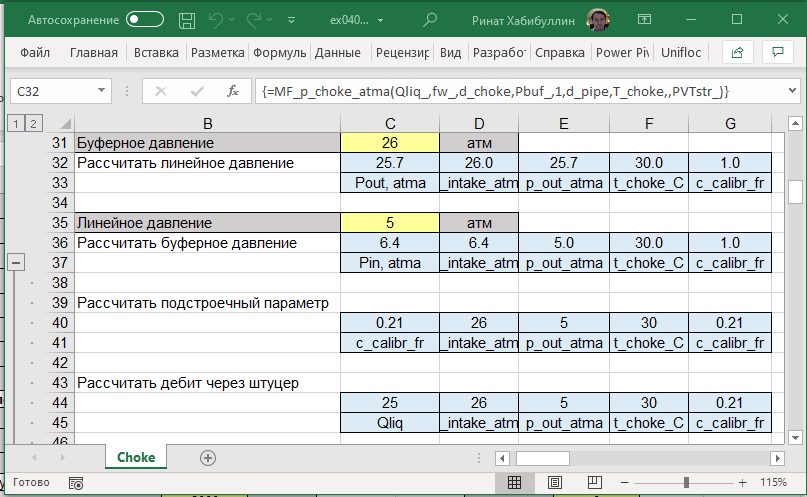
\includegraphics[width=1\linewidth]{choke_array_out}}
	\caption{Пример вывода результата расчета в массив}
	\label{ris:choke_array_out}
\end{figure}


\subsection{MF\_p\_choke\_atma – Расчет давления на входе или на выходе штуцера}
Функция позволяет рассчитать давление на входе или выходе штуцера по известному давлению на противоположном конце при известных параметрах потока (дебите жидкости, обводнённости, газовому фактору). Расчёт проводится по корреляции Перкинса \cite{Perkins_1993} с учётом многофазного потока. 
 
\putlisting{listings/MF_p_choke_atma.lst}



%\subsection{MF\_dp\_choke\_atm – Расчёт перепада давления в штуцере}
%Функция позволяет рассчитать по известному линейному давлению и дебиту или по известному буферному давлению и дебиту перепад давления.  Расчет проводится по корреляции Перкинса \cite{Perkins_1993} с учетом многофазного потока.  
%Функция возвращает перепад давления и температуры в виде массива.
%\putlisting{listings/MF_dp_choke_atm.lst}


\subsection{MF\_qliq\_choke\_sm3day – функция расчёта дебита жидкости через штуцер}
Функция позволяет рассчитать по известному буферному давлению и линейному давлению дебит жидкости. Расчет проводится по корреляции Перкинса \cite{Perkins_1993} с учетом многофазного потока.  

\putlisting{listings/MF_qliq_choke_sm3day.lst}


\subsection{MF\_calibr\_choke\_fr – функция настройки модели штуцера}
Функция позволяет рассчитать корректирующий фактор для модели штуцера, позволяющий согласовать результаты замеров давления и дебита. Расчет проводится по корреляции Перкинса \cite{Perkins_1993} с учетом многофазного потока.  

\putlisting{listings/MF_calibr_choke_fr.lst}

\newpage
\section{Расчет многофазного потока в трубе}

Для расчета участка трубы с использованием пользовательских функций \unf{} применяется схема показанная на рисунке - \ref{ris:Pipe_scheme_1}.

Участок трубы задается как прямой с постоянным наклоном $\theta$  длиной $L$, постоянного диаметра $d$. Поток движется под углом $\theta$ к горизонтальной плоскости. Угол  $\theta$ меняется от -90 до 90 градусов Цельсия. Отрицательная величина  $\theta < 0 $ означает, что поток движется вниз - например отрицательным будет угол наклона для нагнетательной скважины. Угол наклона $\theta = 0 $ соответствует потоку в горизонтальном участке трубопровода.

Труба имеет постоянную по всей длине шероховатость стенок. Шероховатость влияет на коэффициент трения при расчете потока и проявляется при относительно больших скоростях потока. Подробнее про шероховатость и трение в потоке жидкости можно почитать в \cite{Bratland_Pipe_Flow_1}

\begin{figure}[h!]
	\begin{center}
		% https://www.mathcha.io/editor# использован для построения картинок

\tikzset{every picture/.style={line width=0.75pt}} %set default line width to 0.75pt        

\begin{tikzpicture}[x=0.75pt,y=0.75pt,yscale=-1,xscale=1]
%uncomment if require: \path (0,395.3333282470703); %set diagram left start at 0, and has height of 395.3333282470703

%Shape: Can [id:dp2899696286091056] 
\draw  [fill={rgb, 255:red, 250; green, 245; blue, 184 }  ,fill opacity=1 ][line width=2.25]  (164.23,345.91) -- (471.15,94.25) .. controls (473.82,92.06) and (481.92,97.51) .. (489.23,106.43) .. controls (496.54,115.34) and (500.3,124.35) .. (497.63,126.55) -- (190.71,378.2)(164.23,345.91) .. controls (166.9,343.71) and (175,349.16) .. (182.31,358.08) .. controls (189.63,367) and (193.39,376.01) .. (190.71,378.2) .. controls (188.03,380.4) and (179.94,374.95) .. (172.62,366.03) .. controls (165.31,357.11) and (161.55,348.1) .. (164.23,345.91) -- cycle ;
%Shape: Arc [id:dp7673222576415257] 
\draw  [draw opacity=0] (213.54,358.73) .. controls (215.72,361.29) and (217.51,364.25) .. (218.76,367.57) .. controls (220.22,371.43) and (220.84,375.4) .. (220.7,379.27) -- (190.71,378.2) -- cycle ; \draw   (213.54,358.73) .. controls (215.72,361.29) and (217.51,364.25) .. (218.76,367.57) .. controls (220.22,371.43) and (220.84,375.4) .. (220.7,379.27) ;
%Straight Lines [id:da2539925089352497] 
\draw    (111.83,289.33) -- (164.23,345.91) ;


%Straight Lines [id:da27080386920459176] 
\draw    (426.06,41.14) -- (471.15,94.25) ;


%Straight Lines [id:da6784647335940455] 
\draw    (138.03,317.62) -- (448.6,67.7) ;


%Straight Lines [id:da42906958912244875] 
\draw    (343.67,226) -- (373,202.37) ;
\draw [shift={(374.56,201.11)}, rotate = 501.14] [color={rgb, 255:red, 0; green, 0; blue, 0 }  ][line width=0.75]    (10.93,-3.29) .. controls (6.95,-1.4) and (3.31,-0.3) .. (0,0) .. controls (3.31,0.3) and (6.95,1.4) .. (10.93,3.29)   ;

%Straight Lines [id:da31602361859897776] 
\draw    (89,379) -- (569.56,379) ;
\draw [shift={(571.56,379)}, rotate = 180] [color={rgb, 255:red, 0; green, 0; blue, 0 }  ][line width=0.75]    (10.93,-3.29) .. controls (6.95,-1.4) and (3.31,-0.3) .. (0,0) .. controls (3.31,0.3) and (6.95,1.4) .. (10.93,3.29)   ;


% Text Node
\draw (233.67,364.33) node   {$\theta $};
% Text Node
\draw (269.67,187.67) node [rotate=-2.44]  {$L$};
% Text Node
\draw (200.33,343.67) node [rotate=-0.74]  {$P_{in}$};
% Text Node
\draw (472.67,120) node [rotate=-0.74]  {$P_{out}$};
% Text Node
\draw (335.67,230.67) node [rotate=-0.61]  {$Q_{liq}$};


\end{tikzpicture}
		\caption{Схема трубы принятая для расчётов с использованием пользовательских функций}
		\label{ris:Pipe_scheme_1}
	\end{center}
\end{figure}

Для расчёта распределения давления в трубе необходимо задать граничное значение давления на одном из концов трубы. Граничное давление всегда задается параметром  \mintinline{vb.net}{P_calc_from_atma}. Температура потока в точке, где задается давление, задается параметром  \mintinline{vb.net}{T_calc_from_C}, температура на другом конце трубы задается параметром \mintinline{vb.net}{T_calc_to_C}.  Возможно два варианта задания условия - по потоку  \ref{ris:Pipe_scheme_2}  \mintinline{vb.net}{calc_along_flow=1}. и против потока  \ref{ris:Pipe_scheme_3} \mintinline{vb.net}{calc_along_flow=0}. 

\begin{figure}[h!]
	\begin{center}
				\tikzset{every picture/.style={line width=0.75pt}} %set default line width to 0.75pt        
		
		\begin{tikzpicture}[x=0.75pt,y=0.75pt,yscale=-1,xscale=1]
		%uncomment if require: \path (0,390); %set diagram left start at 0, and has height of 390
		
		%Shape: Can [id:dp7382807235009181] 
		\draw  [fill={rgb, 255:red, 250; green, 245; blue, 184 }  ,fill opacity=1 ][line width=2.25]  (176.23,350.28) -- (483.15,98.62) .. controls (485.82,96.43) and (493.92,101.88) .. (501.23,110.8) .. controls (508.54,119.72) and (512.3,128.72) .. (509.63,130.92) -- (202.71,382.57)(176.23,350.28) .. controls (178.9,348.08) and (187,353.54) .. (194.31,362.45) .. controls (201.63,371.37) and (205.39,380.38) .. (202.71,382.57) .. controls (200.03,384.77) and (191.94,379.32) .. (184.62,370.4) .. controls (177.31,361.48) and (173.55,352.47) .. (176.23,350.28) -- cycle ;
		%Shape: Arc [id:dp26711502457409386] 
		\draw  [draw opacity=0] (225.54,363.1) .. controls (227.72,365.66) and (229.51,368.62) .. (230.76,371.95) .. controls (232.22,375.8) and (232.84,379.77) .. (232.7,383.64) -- (202.71,382.57) -- cycle ; \draw   (225.54,363.1) .. controls (227.72,365.66) and (229.51,368.62) .. (230.76,371.95) .. controls (232.22,375.8) and (232.84,379.77) .. (232.7,383.64) ;
		%Straight Lines [id:da2708011557353165] 
		\draw    (123.83,293.7) -- (176.23,350.28) ;
		
		
		%Straight Lines [id:da09547020181005683] 
		\draw    (438.06,45.51) -- (483.15,98.62) ;
		
		
		%Straight Lines [id:da29893852101776] 
		\draw    (150.03,321.99) -- (460.6,72.07) ;
		
		
		%Straight Lines [id:da6573662742713218] 
		\draw    (355.67,230.37) -- (385,206.74) ;
		\draw [shift={(386.56,205.48)}, rotate = 501.14] [color={rgb, 255:red, 0; green, 0; blue, 0 }  ][line width=0.75]    (10.93,-3.29) .. controls (6.95,-1.4) and (3.31,-0.3) .. (0,0) .. controls (3.31,0.3) and (6.95,1.4) .. (10.93,3.29)   ;
		
		%Straight Lines [id:da5485107193914818] 
		\draw    (101,383.37) -- (581.56,383.37) ;
		\draw [shift={(583.56,383.37)}, rotate = 180] [color={rgb, 255:red, 0; green, 0; blue, 0 }  ][line width=0.75]    (10.93,-3.29) .. controls (6.95,-1.4) and (3.31,-0.3) .. (0,0) .. controls (3.31,0.3) and (6.95,1.4) .. (10.93,3.29)   ;
		
		%Right Arrow [id:dp6841435853741948] 
		\draw  [fill={rgb, 255:red, 245; green, 166; blue, 35 }  ,fill opacity=1 ] (135.99,250.8) -- (380.02,50.35) -- (378.16,48.09) -- (395.29,41.6) -- (385.59,57.14) -- (383.73,54.88) -- (139.71,255.32) -- cycle ;
		
		% Text Node
		\draw (245.67,368.7) node   {$\theta $};
		% Text Node
		\draw (281.67,192.04) node [rotate=-2.44]  {$L$};
		% Text Node
		\draw (207.33,354.04) node [rotate=-0.74]  {$P_{in}$};
		% Text Node
		\draw (487.67,117.37) node [rotate=-0.74]  {$P_{out}$};
		% Text Node
		\draw (347.67,235.04) node [rotate=-0.61]  {$Q_{liq}$};
		% Text Node
		\draw  [color={rgb, 255:red, 0; green, 0; blue, 0 }  ,draw opacity=1 ][fill={rgb, 255:red, 245; green, 166; blue, 35 }  ,fill opacity=1 ]  (107, 268.37) circle [x radius= 25.3, y radius= 25.3]   ;
		\draw (107,268.37) node [scale=1.2,rotate=-359.71]  {$P_{calc}$};
		% Text Node
		\draw  [fill={rgb, 255:red, 245; green, 166; blue, 35 }  ,fill opacity=1 ]  (417.67, 24.37) circle [x radius= 23.2, y radius= 23.2]   ;
		\draw (417.67,24.37) node [scale=1.2,rotate=-0.74]  {$P_{out}$};
		
		
		\end{tikzpicture}		
		\caption{Схема расчёта распределения давления по потоку \mintinline{vb.net}{calc_along_flow=1}}
		\label{ris:Pipe_scheme_2}
	\end{center}
\end{figure} 

Схема расчета распределения давления по потоку для случая вертикальной добывающей скважины соответствует расчету распределения давления "снизу вверх" - от забойного давления к устьевому.

\begin{figure}[h!]
	\begin{center}
			
	\tikzset{every picture/.style={line width=0.75pt}} %set default line width to 0.75pt        
	
	\begin{tikzpicture}[x=0.75pt,y=0.75pt,yscale=-1,xscale=1]
	%uncomment if require: \path (0,453); %set diagram left start at 0, and has height of 453
	
	%Shape: Can [id:dp7385102204739014] 
	\draw  [fill={rgb, 255:red, 250; green, 245; blue, 184 }  ,fill opacity=1 ][line width=2.25]  (198.23,370.28) -- (505.15,118.62) .. controls (507.82,116.43) and (515.92,121.88) .. (523.23,130.8) .. controls (530.54,139.72) and (534.3,148.72) .. (531.63,150.92) -- (224.71,402.57)(198.23,370.28) .. controls (200.9,368.08) and (209,373.54) .. (216.31,382.45) .. controls (223.63,391.37) and (227.39,400.38) .. (224.71,402.57) .. controls (222.03,404.77) and (213.94,399.32) .. (206.62,390.4) .. controls (199.31,381.48) and (195.55,372.47) .. (198.23,370.28) -- cycle ;
	%Shape: Arc [id:dp4602786709186524] 
	\draw  [draw opacity=0] (247.54,383.1) .. controls (249.72,385.66) and (251.51,388.62) .. (252.76,391.95) .. controls (254.22,395.8) and (254.84,399.77) .. (254.7,403.64) -- (224.71,402.57) -- cycle ; \draw   (247.54,383.1) .. controls (249.72,385.66) and (251.51,388.62) .. (252.76,391.95) .. controls (254.22,395.8) and (254.84,399.77) .. (254.7,403.64) ;
	%Straight Lines [id:da5353213855148988] 
	\draw    (145.83,313.7) -- (198.23,370.28) ;
	
	
	%Straight Lines [id:da6371642797081225] 
	\draw    (460.06,65.51) -- (505.15,118.62) ;
	
	
	%Straight Lines [id:da5708425902799406] 
	\draw    (172.03,341.99) -- (482.6,92.07) ;
	
	
	%Straight Lines [id:da5694938455522887] 
	\draw    (377.67,250.37) -- (407,226.74) ;
	\draw [shift={(408.56,225.48)}, rotate = 501.14] [color={rgb, 255:red, 0; green, 0; blue, 0 }  ][line width=0.75]    (10.93,-3.29) .. controls (6.95,-1.4) and (3.31,-0.3) .. (0,0) .. controls (3.31,0.3) and (6.95,1.4) .. (10.93,3.29)   ;
	
	%Straight Lines [id:da47656732513988986] 
	\draw    (123,403.37) -- (603.56,403.37) ;
	\draw [shift={(605.56,403.37)}, rotate = 180] [color={rgb, 255:red, 0; green, 0; blue, 0 }  ][line width=0.75]    (10.93,-3.29) .. controls (6.95,-1.4) and (3.31,-0.3) .. (0,0) .. controls (3.31,0.3) and (6.95,1.4) .. (10.93,3.29)   ;
	
	%Right Arrow [id:dp49730840239995544] 
	\draw  [fill={rgb, 255:red, 245; green, 166; blue, 35 }  ,fill opacity=1 ] (419.38,64.16) -- (174.9,264.05) -- (176.75,266.31) -- (159.61,272.77) -- (169.34,257.26) -- (171.19,259.52) -- (415.67,59.63) -- cycle ;
	
	% Text Node
	\draw (267.67,388.7) node   {$\theta $};
	% Text Node
	\draw (303.67,212.04) node [rotate=-2.44]  {$L$};
	% Text Node
	\draw (229.33,374.04) node [rotate=-0.74]  {$P_{in}$};
	% Text Node
	\draw (509.67,137.37) node [rotate=-0.74]  {$P_{out}$};
	% Text Node
	\draw (369.67,255.04) node [rotate=-0.61]  {$Q_{liq}$};
	% Text Node
	\draw  [color={rgb, 255:red, 0; green, 0; blue, 0 }  ,draw opacity=1 ][fill={rgb, 255:red, 245; green, 166; blue, 35 }  ,fill opacity=1 ]  (444, 43.37) circle [x radius= 25.3, y radius= 25.3]   ;
	\draw (444,43.37) node [scale=1.2,rotate=-359.71]  {$P_{calc}$};
	% Text Node
	\draw  [fill={rgb, 255:red, 245; green, 166; blue, 35 }  ,fill opacity=1 ]  (129.67, 288.37) circle [x radius= 21.57, y radius= 21.57]   ;
	\draw (129.67,288.37) node [scale=1.2,rotate=-0.74]  {$P_{in}$};
	
	
	\end{tikzpicture}
		\caption{Схема расчета распределения давления против потока \mintinline{vb.net}{calc_along_flow=0}}
		\label{ris:Pipe_scheme_3}
	\end{center}
\end{figure} 

Схема расчета распределения давления против потока для случая вертикальной добывающей скважины соответствует расчету распределения давления "сверху вниз" - от устьевого давления к забойному.
Все функции для расчета штуцера содержат в названии слово \mintinline{vb.net}{pipe}.

%\subsection{MF\_dp\_pipe\_atm – расчёт перепада давления в трубе}

%Функция позволяет рассчитать перепад давления в участке трубопровода. 
%Функция возвращает давление и температуру в виде массива.

%\putlisting{listings/MF_dp_pipe_atm.lst}

Ниже на рисунке \ref{ris:VLP_curves} приведены результаты расчёта кривой оттока (перепада давления в вертикальной трубе) для различных корреляций, реализованных в \unf{}.

\begin{figure}[h!]
	\begin{center}
	\newcommand{\dPipeDataFile}{data/dPipe.txt}
		\begin{tikzpicture}[scale=1]
		\begin{axis}[
					width=14cm,
					height=10cm,
					xlabel=$Q\; m^3 / day$,
					ylabel=$P_{wf} \; atma$,
					legend pos=south east,
					title=Pipe Pressure Drop]
		\addplot table [y=P_0, x=Q]{\dPipeDataFile};
		\addlegendentry{Beggs Brill}
		\addplot table [y=P_1, x=Q]{\dPipeDataFile};
		\addlegendentry{Ansari}
		\addplot table [y=P_2, x=Q]{\dPipeDataFile};
		\addlegendentry{Unified}
		\addplot table [y=P_3, x=Q]{\dPipeDataFile};
		\addlegendentry{Gray}
		\addplot table [y=P_4, x=Q]{\dPipeDataFile};
		\addlegendentry{Hagedorn Brown}
		\addplot table [y=P_5, x=Q]{\dPipeDataFile};
		\addlegendentry{Sakharov Mokhov}
		\end{axis}
		\end{tikzpicture}	
	\caption{Кривые характеристики многофазного потока для вертикальных труб рассчитанные с использованием различных корреляций }
	\label{ris:VLP_curves}
	\end{center}
\end{figure}

\subsection{MF\_p\_pipe\_atma – функция расчета давления на конце трубы}  
Функция позволяет рассчитать перепад давления в участке трубопровода. Функция обеспечивает несколько режимов расчёта. Некоторые особенности работы функции \mintinline{vb.net}{MF_p_pipe_atma()}
\begin{itemize}
	\item Свойства флюида в трубе определяются параметром \mintinline{vb.net}{str_PVT}, который в свою очередь может быть задан функцией \mintinline{vb.net}{PVT_encode()}.
	\item Дополнительно в поток может быть включен свободный газ. Задается параметром \mintinline{vb.net}{q_gas_sm3day} определяющим объемный расход приведенный к стандартным условиям. Свободный газ суммируется с газом определяемым исходя из заданных свойств флюида. 
	\item Если при определении \mintinline{vb.net}{str_PVT} указан параметр \mintinline{vb.net}{gas_only = 1}, то расчет распределения давления в трубе будет проводиться для газа, наличие жидкости в потоке учитываться не будет. В текущей версии \unf{} при расчете потока газа трение газа не учитывается, перепад давления в газовой линии не зависит от расхода газа, зависит только от плотности газа.
	\item Если параметр дебита жидкости  \mintinline{vb.net}{qliq_sm3day = 0}  равен нулю, расчет проводится для режима барботажа (ZNLF - zero net liquid flow) - движения газа через неподвижный столб жидкости. Расход газа должен быть задан параметром \mintinline{vb.net}{q_gas_sm3day}. В текущей версии \unf{} расчет барботажа проводится проводится за счет переключения на механистическую корреляцию Ансари. Попытка построить график зависимости перепад давления от дебита для других корреляций может дать нелогичный результат около нулевого дебита (скачек перепада давления). Рекомендуется без необходимости для \mintinline{vb.net}{qliq_sm3day = 0} не считать при построении графиков.
	\item Распределение температуры для функции расчета участка скважины ограничено одной моделью - линейного распределения температуры потока вдоль трубы. Для учета температуры необходимо задать параметры \mintinline{vb.net}{t_calc_from_C} и \mintinline{vb.net}{t_calc_to_C} определяющие температуру на концах трубы. В трубе значения будут проинтерполированы по длине. Если второй параметр \mintinline{vb.net}{t_calc_to_C} не задать, то температура в трубе будет постоянной. Проконтролировать расчет температуры можно воспользовавшись выводом результатов расчета в виде массива.
\end{itemize}
 

Результатом работы функций является массив значений содержащий давление и температуру флюида на входе в трубу $P_{in}, T_{in}$, давление и температуру флюида на выходе из трубы $P_{out}, T_{out}$,  калибровочные коэффициент многофазной корреляции для гравитационной состовляющей и для трения$c_{calibr\_grav},c_{calibr\_fric}$.  Выходной массив содержит две строки - в первой находятся значения, во второй подписи. Это позволяет при необходимости вывести только значения в той же строке в которой проводился расчет. Значение в первой строке и в первом столбце зависит от настройки функции (параметра \mintinline{vb.net}{calc_along_flow} для функции \mintinline{vb.net}{MF_p_pipe_atma}) и содержит основной результат расчета. Значения в последующих столбцах не зависят от настройки функции и показывают все результаты расчета.
Для вывода массива в Excel следует выбрать необходимый диапазон ячеек, в который будут выводится результаты в виде массива, затем ввести в адресную строку вызов функции и нажать комбинацию клавиш - Cntrl-Shift-Enter. После этого название функции в адресной строке должно отображаться в фигурных скобках, аналогично функции расчета давления в штуцере, рисунок \ref{ris:choke_array_out}. При необходимости внести коррективы в вызов функции также необходимо подтверждать свои действия комбинацией клавиш Cntrl-Shift-Enter.

\putlisting{listings/MF_p_pipe_atma.lst}

\subsection{MF\_calibr\_pipe\_m3day - функция калибровки расчета участка трубы}

\putlisting{listings/MF_calibr_pipe_m3day.lst}

%\subsection{MF\_p\_pipe\_znlf\_atma – функция расчета давления на конце трубы при барботаже}  
% отдельной функции для барботажа больше нет - если дебит задать ноль то и MF_p_pipe_atma будет считать барботаж
%
%\putlisting{listings/MF_p_pipe_znlf_atma.lst}

\subsection{MF\_dpdl\_atmm – функция расчета градиента давления по многофазной корреляции}  

\putlisting{listings/MF_dpdl_atmm.lst}

\newpage

